\documentclass[11pt]{article}
\usepackage[margin=1in]{geometry}
\usepackage{amsmath,amssymb,amsthm,mathtools}
\usepackage{graphicx}
\usepackage{microtype}
\usepackage[hidelinks]{hyperref}
\usepackage{enumitem}

\newtheorem{theorem}{Theorem}
\newtheorem{proposition}[theorem]{Proposition}
\newtheorem{lemma}[theorem]{Lemma}
\newcommand{\C}{\mathbb C}
\newcommand{\R}{\mathbb R}
\newcommand{\Sph}{\mathbb S}
\newcommand{\Vol}{\mathrm V}
\newcommand{\F}{\mathbf F}
\newcommand{\I}{\mathrm I}
\newcommand{\Kc}{\mathcal K}
\newcommand{\pair}[2]{\langle #1,#2\rangle}

\title{A Sharp Ellipse Dichotomy for a Complex\\
Busemann--Petty Problem}
\author{Automated mathematics run \texttt{fa\_banach\_001}, lane 0}
\date{August 11, 2026}

\begin{document}
\maketitle

\begin{center}
\fbox{\parbox{0.91\textwidth}{\textbf{Status.}
Candidate full counterexample theorem, likely valid, pending expert review.
For every $-2<p<0$, the Busemann--Petty implication for the complex
$L_p$-intersection operator in $\C^2$ is affirmative for circular planar
ellipses and negative for every noncircular origin-centered ellipse.}}
\end{center}

\section{Source problem and the untreated case}

Ellmeyer and Hofst\"atter~\cite{EH} define complex $L_p$-intersection
operators $\I_{C,p}$ for an origin-symmetric planar convex body
$C\subset\C$ and ask their general Busemann--Petty Problem~1:
for $K,L$ in the injectivity set $\Kc(\I_{C,p})$, does
\begin{equation}\label{eq:BP}
 \I_{C,p}K\subseteq\I_{C,p}L
 \quad\Longrightarrow\quad
 \Vol_4(K)\le \Vol_4(L)
\end{equation}
hold?  The source proves that for $-2<p<0$ the answer in complex dimension
two is affirmative when $C$ is the disk.  Its main theorem does not treat
general $C$ in that dimension; the introduction explains that the image is
described completely only for the disk.

\begin{figure}[ht]
  \centering
  
\includegraphics[width=\textwidth]{figures/open_problem_crop.png}
  \caption{Problem~1 on page 2 of arXiv:2404.05630v3.}
  \label{fig:problem}
\end{figure}

\begin{figure}[ht]
  \centering
  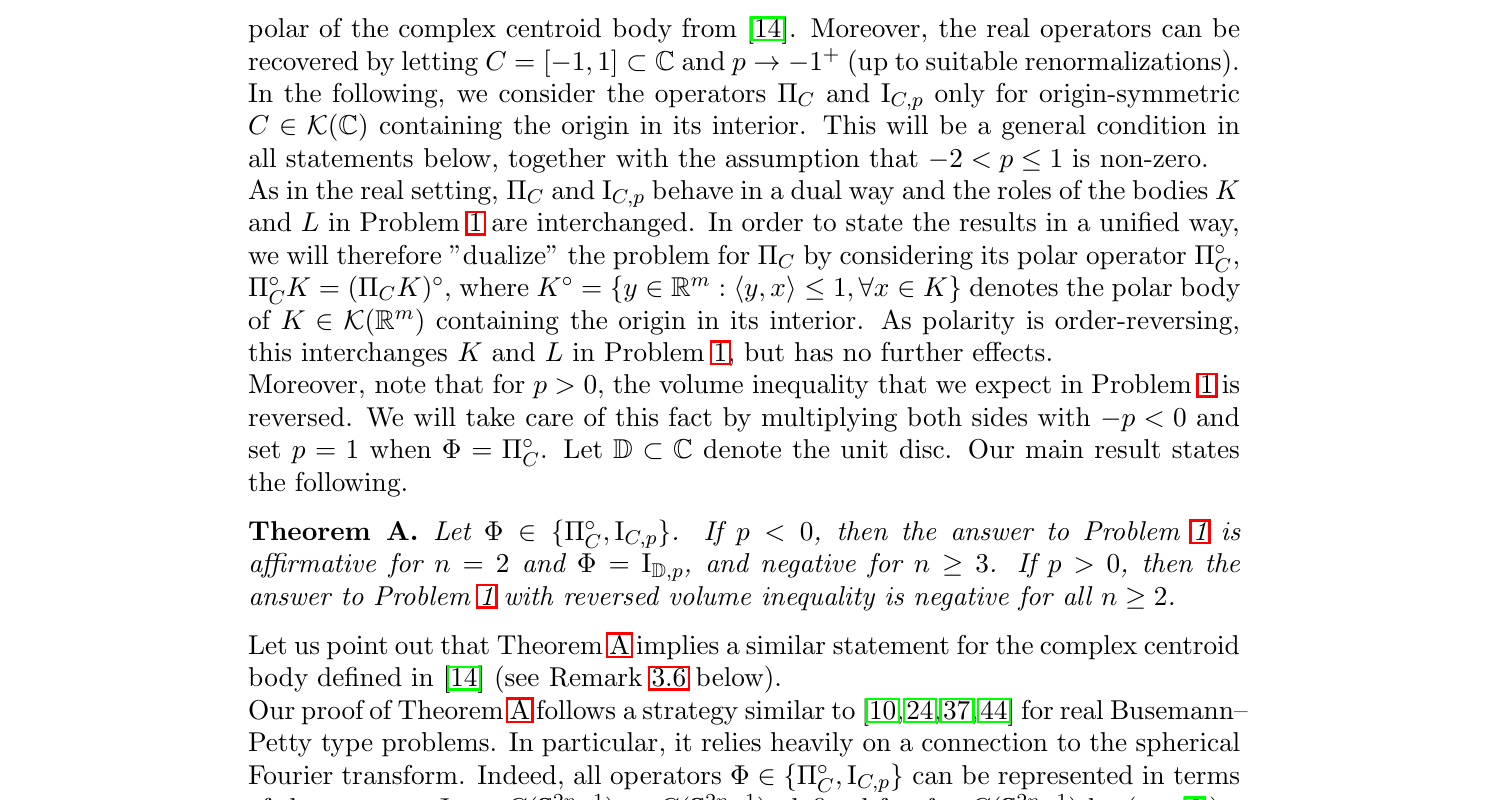
\includegraphics[width=\textwidth]{figures/source_scope_crop.png}
  \caption{Theorem A on page 3 singles out the disk in complex dimension two.}
  \label{fig:scope}
\end{figure}

The result below fills this gap for every origin-centered ellipse.  It also
shows that the disk theorem is unstable: an arbitrarily small noncircular
elliptic deformation reverses the answer.

\section{Source identities and notation}

Write $m=4$ and let $\F_q$ be the spherical Fourier transform of degree $q$
on even functions on $\Sph^3$, with the normalization of~\cite{EH}.  For a
finite measure $\nu$ on $\Sph^1$, set
\[
 (T_\nu f)(u)=\int_{\Sph^1}f(cu)\,d\nu(c).
\]
The source proves that
\begin{equation}\label{eq:source-transform}
 \rho_{\I_{C,p}K}^{-p}
 =\frac{1}{(2\pi)^2(4+p)}
 T_{\nu_{C,p}}\F_{-4-p}\rho_K^{4+p},
 \qquad \nu_{C,p}=\F_p h_C^p,
\end{equation}
where $\nu_{C,p}$ is a positive nonzero even measure for $p<0$.  It also
proves
\begin{equation}\label{eq:inverse}
 \F_{-4-p}\F_p f=(2\pi)^4f,
\end{equation}
and that the transforms are self-adjoint.

The injectivity set is characterized by the angular Fourier coefficients:
an origin-symmetric body belongs to $\Kc(\I_{C,p})$ exactly when every
harmonic component of $\rho_K^{4+p}$ corresponding to a zero coefficient of
$h_C^p$ vanishes.  In particular, if all even Fourier coefficients of
$h_C^p$ are nonzero, $\Kc(\I_{C,p})$ is the set of all origin-symmetric
convex bodies with nonempty interior.

Finally, for star bodies in $\R^4$ the dual mixed volume is
\[
 \widetilde V_{-p}(K,L)
 =\frac14\int_{\Sph^3}\rho_K^{4+p}\rho_L^{-p},
\]
and the dual $L_p$-Minkowski inequality used in~\cite{EH} says
\begin{equation}\label{eq:dual-minkowski}
 -p\widetilde V_{-p}(K,L)
 \le -p\Vol_4(K)^{(4+p)/4}\Vol_4(L)^{-p/4}.
\end{equation}

\section{Proof intuition}

The disk kills every non-$\Sph^1$-invariant angular harmonic, so its
injectivity set contains only balanced bodies.  A noncircular ellipse does the
opposite: every even angular multiplier is nonzero, hence all
origin-symmetric bodies are admissible.

This permits a sign-changing perturbation.  On a real Lagrangian plane
$E\subset\C^2$, choose an even function $\varphi$ which is negative on
$\Sph^3\cap E$, but whose positive angular convolution
$T_{\nu_{C,p}}\varphi$ is strictly positive everywhere.  A thin real
ellipsoid has $L_p$-embedding measure concentrated on that circle, so the
pairing of $\varphi$ with the measure is negative.  Perturbing the radial
power of the ellipsoid by $\F_p\varphi$ makes the transformed body smaller
pointwise, while the dual mixed-volume calculation makes its ordinary volume
strictly larger.  These are exactly the two inequalities needed for a
counterexample.

\section{The ellipse dichotomy}

\begin{theorem}[sharp dichotomy among ellipses]\label{thm:main}
Fix $-2<p<0$, and let $C\subset\C$ be an origin-centered ellipse with
nonempty interior.
\begin{enumerate}[label=\textup{(\roman*)}]
\item If $C$ is a disk up to dilation, implication~\eqref{eq:BP} holds.
\item If $C$ is noncircular, there are smooth origin-symmetric strictly
convex bodies $K,L\subset\C^2$ in $\Kc(\I_{C,p})$ such that
\[
 \I_{C,p}K\subsetneq\I_{C,p}L
 \qquad\text{and}\qquad
 \Vol_4(K)>\Vol_4(L).
\]
\end{enumerate}
Thus the disk is the unique affirmative ellipse for every exponent in the
entire interval $(-2,0)$.
\end{theorem}

Part (i) is Theorem A and Proposition 1.5 of~\cite{EH}; dilating $C$ merely
rescales the operator.  We prove part (ii) in four steps.

\subsection{Every even ellipse multiplier is nonzero}

After a rotation and dilation, the support function of a noncircular ellipse
satisfies
\[
 h_C(e^{i\theta})^2=A+B\cos(2\theta),
 \qquad A>|B|>0,\quad B\ne0.
\]
Put $s=-p/2>0$.  For $j\ge0$, the Fourier coefficient at frequency $2j$ of
$h_C^p$ is, up to a nonzero normalization, the coefficient at frequency $j$
of $(A+B\cos x)^{-s}$.  The Laplace representation gives
\begin{align*}
 (A+B\cos x)^{-s}
 &=\frac1{\Gamma(s)}\int_0^\infty
 t^{s-1}e^{-At}e^{-Bt\cos x}\,dt,\\
 \widehat{h_C^p}(2j)
 &=\frac{(-\operatorname{sgn}B)^j}{\Gamma(s)}
 \int_0^\infty t^{s-1}e^{-At}I_j(|B|t)\,dt,
\end{align*}
again up to a fixed positive normalization.  The modified Bessel function
$I_j(t)$ is strictly positive for $t>0$, so this coefficient never vanishes.
Origin symmetry kills only the odd coefficients, which are irrelevant for
even data.  Consequently $\I_{C,p}$ is injective on every even function and
\begin{equation}\label{eq:inj-all}
 \Kc(\I_{C,p})
 =\{\text{all origin-symmetric convex bodies with nonempty interior}\}.
\end{equation}

\subsection{A sign-changing function with positive angular image}

The same ellipse can be written $h_C(x)=|Bx|$ on $\R^2$ for an invertible
real matrix $B$.  The standard Fourier formula for homogeneous Euclidean
powers~\cite[Chapter 3]{Koldobsky} and a linear change of variables give
\begin{equation}\label{eq:nu-density}
 d\nu_{C,p}(c)
 =\kappa_p|\det B|^{-1}|B^{-T}c|^{-2-p}\,dc,
 \qquad \kappa_p>0.
\end{equation}
Thus $\nu=\nu_{C,p}$ has a positive continuous density on $\Sph^1$.
Let
\[
 M=\nu(\Sph^1),
 \qquad
 r=\frac1M\left|\int_{\Sph^1}c^2\,d\nu(c)\right|<1.
\]
The strict inequality follows from equality in the triangle inequality: since
the density is positive everywhere, $c^2$ is not constant on its support.

Take the real Lagrangian plane $E=\R^2\subset\C^2$ and define
\[
 Q(u)=|P_Eu|^2,\qquad u\in\Sph^3.
\]
Writing $u=x+iy$ with $x,y\in E$ and $c=e^{i\theta}$,
\[
 Q(cu)=\frac12+\frac{|x|^2-|y|^2}{2}\cos(2\theta)
                 -\pair{x}{y}\sin(2\theta).
\]
The amplitude of the second harmonic is at most $1/2$, because
\[
 (|x|^2-|y|^2)^2+4\pair{x}{y}^2
 \le (|x|^2+|y|^2)^2=1.
\]
It follows that
\begin{equation}\label{eq:TQ}
 T_\nu Q(u)\le \frac{M(1+r)}2
 \qquad (u\in\Sph^3).
\end{equation}
Choose
\begin{equation}\label{eq:a-choice}
 1<a<\frac{2}{1+r},
 \qquad \varphi=1-aQ.
\end{equation}
Then $\varphi$ is smooth and even,
\begin{equation}\label{eq:witness-signs}
 T_\nu\varphi
 \ge M\left(1-\frac{a(1+r)}2\right)>0,
 \qquad
 \varphi|_{\Sph^3\cap E}=1-a<0.
\end{equation}

\subsection{An embedding measure concentrated on the negative circle}

Let $F=iE$ and, for $0<\delta<1$, set
\[
 A_\delta=\delta P_E+P_F,
 \qquad L_\delta=A_\delta B_2^4.
\]
This is a smooth strictly convex origin-symmetric ellipsoid.  Since
$\rho_{L_\delta}^{-p}(u)=\|u\|_{L_\delta}^{p}$, another linear change in the
Fourier transform yields the positive density
\begin{equation}\label{eq:mu-delta}
 d\mu_\delta(u):=d(\F_p\rho_{L_\delta}^{-p})(u)
 =\gamma_p\delta^2
 \bigl(\delta^2|P_Eu|^2+|P_Fu|^2\bigr)^{-(4+p)/2}\,du,
 \quad \gamma_p>0.
\end{equation}

The normalized measures $\mu_\delta/\mu_\delta(\Sph^3)$ concentrate on
$\Sph^3\cap E$ as $\delta\downarrow0$.  Here is a direct check.  Under uniform
measure on $\Sph^3$, the variable $t=|P_Eu|^2$ is uniform on $[0,1]$; hence,
up to a positive constant, the density in $t$ is
\[
 \delta^2(\delta^2t+1-t)^{-\alpha},
 \qquad \alpha=\frac{4+p}{2}\in(1,2).
\]
Outside any fixed neighborhood of $t=1$ its mass is $O(\delta^2)$.  On
$1-\delta^2\le t\le1$ its mass is bounded below by a constant times
$\delta^{4-2\alpha}=\delta^{-p}$.  Since $2+p>0$, the ratio tends to zero.
This proves concentration.  By~\eqref{eq:witness-signs}, therefore,
\begin{equation}\label{eq:negative-pairing}
 \frac{\pair{\varphi}{\mu_\delta}}
      {\mu_\delta(\Sph^3)}\longrightarrow1-a<0.
\end{equation}
Fix $\delta$ small enough that $\pair{\varphi}{\mu_\delta}<0$, and write
$L=L_\delta$.

\subsection{The radial perturbation}

Let $\psi=\F_p\varphi$.  For $\varepsilon>0$ define a star body $K$ by
\begin{equation}\label{eq:K-def}
 \rho_K^{4+p}=\rho_L^{4+p}-\varepsilon\psi.
\end{equation}
For sufficiently small $\varepsilon$, the right side is positive and $K$ is
smooth and strictly convex.  This is the standard radial perturbation lemma
used as Lemma 3.1 in~\cite{EH}; strict positive curvature is open under the
resulting $C^2$ perturbation of the ellipsoid.  Both bodies are
origin-symmetric, so~\eqref{eq:inj-all} puts $K,L$ in the required
injectivity set.

Apply~\eqref{eq:source-transform},~\eqref{eq:inverse}, and
~\eqref{eq:witness-signs}:
\begin{align*}
 \rho_{\I_{C,p}K}^{-p}
 &=\rho_{\I_{C,p}L}^{-p}
 -\varepsilon\frac{(2\pi)^2}{4+p}T_\nu\varphi
 <\rho_{\I_{C,p}L}^{-p}.
\end{align*}
Because $-p>0$, this is equivalent to the strict radial inclusion
$\I_{C,p}K\subsetneq\I_{C,p}L$.

For the volume sign, self-adjointness of $\F_p$ and
~\eqref{eq:negative-pairing} give
\begin{align*}
 -4p\widetilde V_{-p}(K,L)
 &=-p\pair{\rho_K^{4+p}}{\rho_L^{-p}}\\
 &=-4p\Vol_4(L)
   +p\varepsilon\pair{\psi}{\rho_L^{-p}}\\
 &=-4p\Vol_4(L)
   +p\varepsilon\pair{\varphi}{\F_p\rho_L^{-p}}
 >-4p\Vol_4(L).
\end{align*}
Combining this strict inequality with~\eqref{eq:dual-minkowski} gives
\[
 -p\Vol_4(L)
 <-p\Vol_4(K)^{(4+p)/4}\Vol_4(L)^{-p/4},
\]
and hence $\Vol_4(K)>\Vol_4(L)$.  This proves Theorem~\ref{thm:main}.

\section{Verification, scope, and novelty}

The proof is analytic; no numerical assertion is used.  The included script
\path{code/numerical_sanity.py} evaluates the explicit one-dimensional
second-moment and concentration integrals for one ellipse and five exponents.
In each case it confirms both strict signs in~\eqref{eq:witness-signs} and
~\eqref{eq:negative-pairing}.  It is only a regression check.

The claim fully classifies origin-centered ellipses, but does not classify all
origin-symmetric planar bodies $C$.  The same argument works whenever all even
coefficients of $h_C^p$ are nonzero and the second angular moment is strict.
Kernels with finite rotational symmetry can have systematic zero multipliers;
then the concentrating real ellipsoid need not belong to the injectivity set,
so a new symmetry-compatible construction is needed.

The novelty search was bounded but current through August 11, 2026.  It
covered the run indexes; exact arXiv-id, title, author, ellipse, and
noncircular-ellipse searches; the current arXiv v3 and published-paper
metadata; the authors' publication list; and their MathOverflow errata page.
No later resolution or ellipse dichotomy was found.  The mechanism uses the
source's Fourier and perturbation framework in a new non-$\Sph^1$-invariant
way, so expert novelty review remains appropriate.

Human review should prioritize four points: the nonvanishing Bessel
coefficient calculation; the normalization-independent strict bound
~\eqref{eq:TQ}; the weak concentration in~\eqref{eq:mu-delta}; and the two
signs in the final dual mixed-volume calculation.

\begin{thebibliography}{9}
\bibitem{EH}
S. Ellmeyer and G. C. Hofst\"atter,
\emph{Busemann--Petty type problems on complex vector spaces},
Indiana Univ. Math. J. \textbf{75} (2026), no.~2, 525--551;
arXiv:2404.05630v3.

\bibitem{Koldobsky}
A. Koldobsky,
\emph{Fourier Analysis in Convex Geometry},
Mathematical Surveys and Monographs 116, American Mathematical Society, 2005.
\end{thebibliography}

\end{document}
